\section{Challenges}
\label{chal}
There are several challenges to be taken into consideration while designing a benchmark for SDPSs. In this section we analyse the challenges and provide solutions.

\para{ \textit{Simple is beautiful}}. The first challenge is to design a simple system for the driver, because this avoids extra overheads and bottlenecks and of course, simple is beautiful. As the number of sub-systems included in driver increases, the complexity escalades at the same time. One of downsides of the complex system is, difficult to determine the bottleneck. One example is the connection system between data generator and SUT.  To test the stream data processing engine, the data generator component is essential, to simulate the real life scenarios. Figure \ref{fig_queue_link} shows possible three cases to link data generator and SUT. The simplest design would be connecting the SDPS directly to data generators as shown in Figure \ref{fig_no_queue}. Although this is perfectly acceptable case, it confronts with real life use cases. That is,  in real life, the stream data processing engines, do not connect to pull based data sources unless there is a specific system design. Usually, SDPSs pull data from the distributed message queues which reside between data sources and SUT as shown in Figure \ref{fig_yes_queue}. One bottleneck of this option is throughput which is bounded by the maximum throughput of message queueing system. Moreover, there is another  de-/serialization layer  which \textit{artificially} increases SUT's latency. We selected the third option which stands between the first two. As can be seen from Figure \ref{fig_partial_queue}, we embedded the queues as a separate module in data generators. In this way, the throughput is bounded only by network bandwidth, the system works more efficiently as there are no de-/serialisation overheads, it can scale out easily and finally it has a simple design. 


\para{ \textit{Isolate driver and test units}}. The second challenge is to isolate the benchmark driver and SUT as much as possible. For example, in SDPSs benchmarks, it is common to measure the throughput inside the SUT. Because both computations (driver and test) can affect each other the results can be  biased  which is discussed below. We solved this problem by categorising the test unit and pointing measurements accordingly. The first evaluation is throughput. Throughput is associated with the system. So, we kept the throughput assessment outside the SUT, inside data generator module. The second evaluation is latency. The latency is linked with an operator inside system. So, we kept all latency measurements outside the particular operator.

\para{ \textit{ Artificial latency and throughout}}.
The third challenge is to abstain from biased test results and keep the evaluation semantics clear.  One example for this is, throughput measurement. In the previous SDPS benchmarks, the throughput of a SUT is measured by either taking quantiles over test time, or showing max, min and average assessments. From user's perspective on the other hand, the system's maximum throughput is  defined as upper bound  for processing the given workload. When conducting the experiments with stream data processing engines, back pressure is one factor affecting the throughput, that should be taken into consideration.  We solve the first issue by measuring the SUT's max throughput with maximum workload that it can sustain. We give the definition of SUT's sustainability with given workload.
The mechanism we provide for measuring sustainability is customisable based on user's preferences. For example, it can take user-defined function and measure sustainability according to particular function. In this way, we can easily plug the custom logic for back-pressure handling. 

 Another example for this challenge is latency measurement. Latency is a time interval between the stimulation and response. For batch data processing systems, we assume that data is already in the system so, the latency is the interval between tuples' read and output. For SDPSs on the other hand, the latency is the time between tuple's event time and output. If there are extra systems between SDPS and data source, then those are likely to add \textit{artificial latency} for each tuple.  Some researchers circumvented this problem by measuring latency in SDPS the same as in batch data processing systems. In this case, the number and complexity of the systems between SDPS and data source is regardless as latency is the interval between tuples' ingestion and output. However, this measure of latency is \textit{optimistic} as latency for SDPSs is between tuple's event time and output time. Another factor triggering the \textit{artificial latency} is input data rate. If the input data rate is higher than the SDPS can sustain, the results can be biased. Even if the system supports back-pressure, if data rate is more than it can sustain, initially the system will try to ingest as much data as possible. Then, the calculation time will take longer and the latency will increase for every tuple. For this case, it is crucial to measure system's sustainability rate and calculate the latency in that specific configuration, otherwise the measurements will be biased.  We solve this issue by clearing the systems creating artificial latency between data source and SDPS and measuring the latency with the sustainable throughput only. 
 


\para{ \textit{ Latency of stateful operator}} The fourth challenge is measuring the latency of stateful operator. Up to this point, the related works in the literature either concentrated on stateless operators or evaluated the latency of stateful operators by checkpointing to external systems like lightweight distributed databases. As we discussed above, this approach can be a bottleneck in some cases. In this paper, we  define the latency of stateful operator formally and  provide a solution for this problem without any external system. Basically, the latency of the target operator can be calculated by just putting extra operator adjacent to it and the difference in tuple's timestamp and current timestamps are calculated in particular operator.

\begin{figure*}
    \centering
    \begin{subfigure}[b]{0.32\textwidth}
        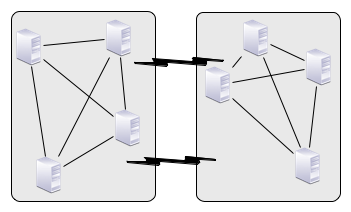
\includegraphics[width=\textwidth]{eps/no_queue}
        \caption{Without message queue}
        \label{fig_no_queue}
    \end{subfigure}
    ~ %add desired spacing between images, e. g. ~, \quad, \qquad, \hfill etc. 
      %(or a blank line to force the subfigure onto a new line)
    \begin{subfigure}[b]{0.32\textwidth}
        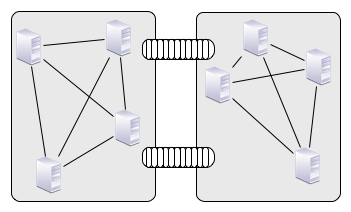
\includegraphics[width=\textwidth]{eps/yes_queue}
        \caption{With message queue}
        \label{fig_yes_queue}
    \end{subfigure}
    \begin{subfigure}[b]{0.32\textwidth}
        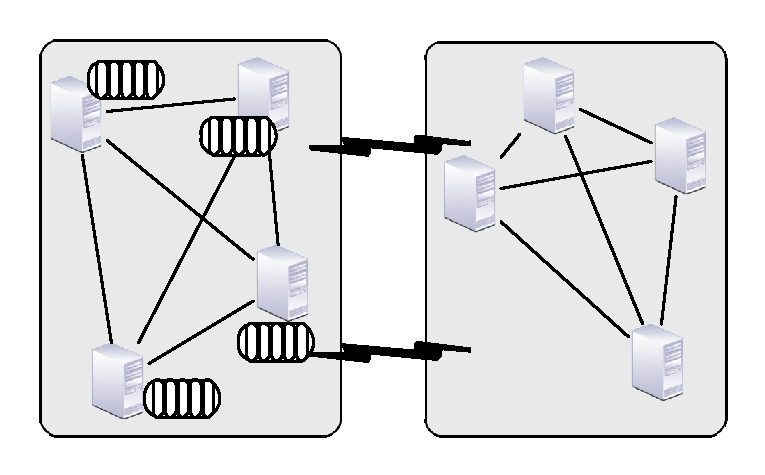
\includegraphics[width=\textwidth]{eps/node_queue}
        \caption{Partial message queue}
        \label{fig_partial_queue}
    \end{subfigure}
        \caption{Different system designs to link data generator and SUT.}
            \label{fig_queue_link}
\end{figure*}
